\section{Der minimalistische Comp}
Es gibt immer mehr Webshops, wo die Seiten mit eigentlich unnötigen Sachen oder Werbung überladen sind. Als Idee hat dieser Webshop-Entwurf, dass die Seite minimalistisch gehalten wird, um so viel wie möglich auszudrücken bei minimalem Design.  
\\
Diese Seite ist durch Responsive Designing auch für Handhelds und Tablets geeignet.
	\subsection{Comprehensive Dummy}
Der zeichnerische Entwurf (siehe Abbildung \ref{mini_comp1}) zeigt schon, wie die Grundidee umgesetzt werden soll. So wurde versucht, diesen in HTML und CSS umzusetzen. Dort traten keine designtechnischen Probleme auf.
\begin{figure} [hp]
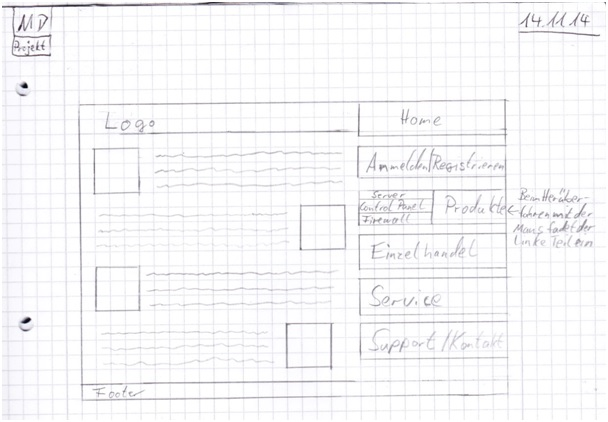
\includegraphics[width=\textwidth]{./img/mini_comp1.png}
\caption{Der Umsetzung der Idee auf Papier}
\label{mini_comp1}
\end{figure}
	\subsection{Entwicklungsphase HTML\&CSS}
Der erste Entwurf des Comps wurde in HTML umgesetzt. Hierbei sah man noch nicht viel von der Strukturierung, wie es im Comprehensive Dummy gedacht ist. Die Elemente waren einfach untereinander angeordnet. (siehe Abbildung  \ref{mini_comp2})
\\
\begin{figure} [hp]
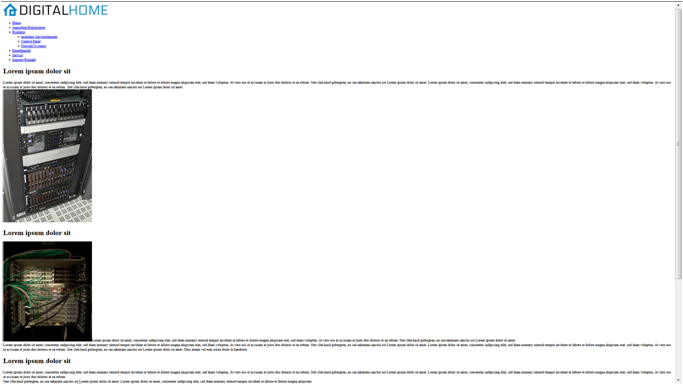
\includegraphics[width=\textwidth]{./img/mini_comp2.png}
\caption{Die erste Umsetzung in HTML}
\label{mini_comp2}
\end{figure}
Als zusätzlich noch CSS implementiert wurde, nahm die Seite ihre Form an, wie sie Comprehensive Dummy sein soll. Hierbei bereitete die Menüleiste Probleme, weil die anfangs noch manche Elemente aus dem Footer, Content und Header überdeckt hat. Da Unterkategorien direkt bei den Navigationspunkten in der vorgesehenen Anordnung nicht funktioniert hat, wurde dies herausgenommen. Die Unterpunkte bekommt man stattdessen dann, wenn man auf den jeweiligen Navigationspunkt drückt im Content-Bereich angezeigt. Der Fehler, wo andere Elemente von der Navigationsleiste überdeckt werden, wurde durch Anpassen der Breiten und Höhen der Elemente beseitigt.
\\
Das Responsive Design bereitete auch Probleme. Dies wurde jedoch behoben, wodurch man, trotz des Entfernens der Unterkategorien, einen sehr originaltreuen Comprehensive Dummy als Webseitenentwurf hat. (siehe Abbildung  \ref{mini_comp3})
\begin{figure} [hp]
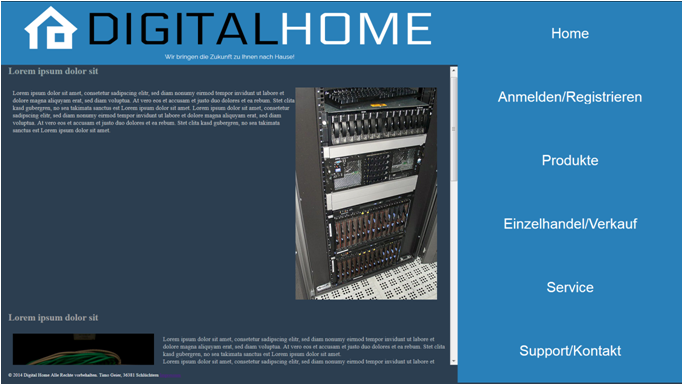
\includegraphics[width=\textwidth]{./img/mini_comp3.png}
\caption{Die endgültige Umsetzung mit HTML und CSS}
\label{mini_comp3}
\end{figure}

	\subsection{Farbgebung}
	\label{farb_mini}
Da der Webshop Digitale Haustechnik verkauft, sollten die Farben offen und sehr intelligent wirken, zudem eine gewisse Ruhe und Kühle ausstrahlen. Aber es sollte auch zum Minimalismus des Seitenaufbaus passen.
\\
\\
Deswegen basiert das Farbschema in der Online-Fassung hauptsächlich auf blauen Farbtönen, wie man in der Abbildung \ref{mini_farb1} zu sehen. Die Hintergrundfarbe und die Footerfarbe sind in einem dunklen Blau, das Ruhe, Konzentration und Sachlichkeit von Informationen symbolisiert. 
Sowohl der Header, als auch die Elemente der Navigationsleiste sind in unterschiedlichen Blautönen, je nachdem, ob man mit dem Cursor über den Header oder die Elemente der Navigationsleiste fährt oder nicht. Sie sollen offen und intelligent wirken. Zusätzlich sind diese Farben im Kontrast zum Hintergrund und Footer, wodurch sie sehr im Fokus stehen.
\\
Die Überschriften und die Texte sind in jeweils zwei unterschiedlichen Grautönen gefärbt. Diese sollen die Sachlichkeit, Funktionalität, Schlichtheit, und den Minimalismus der Seite ausdrücken. Zudem kann man die Absätze dadurch besser voneinander unterscheiden.
\\
Die Schriftfarbe des Footers ist weiß, damit man den sehr gut lesen, denn er enthält wichtige Informationen zum Copyright, dem Webseitenbetreiber und zudem den Link zum Impressum der Seite. 
\begin{figure} [hp]
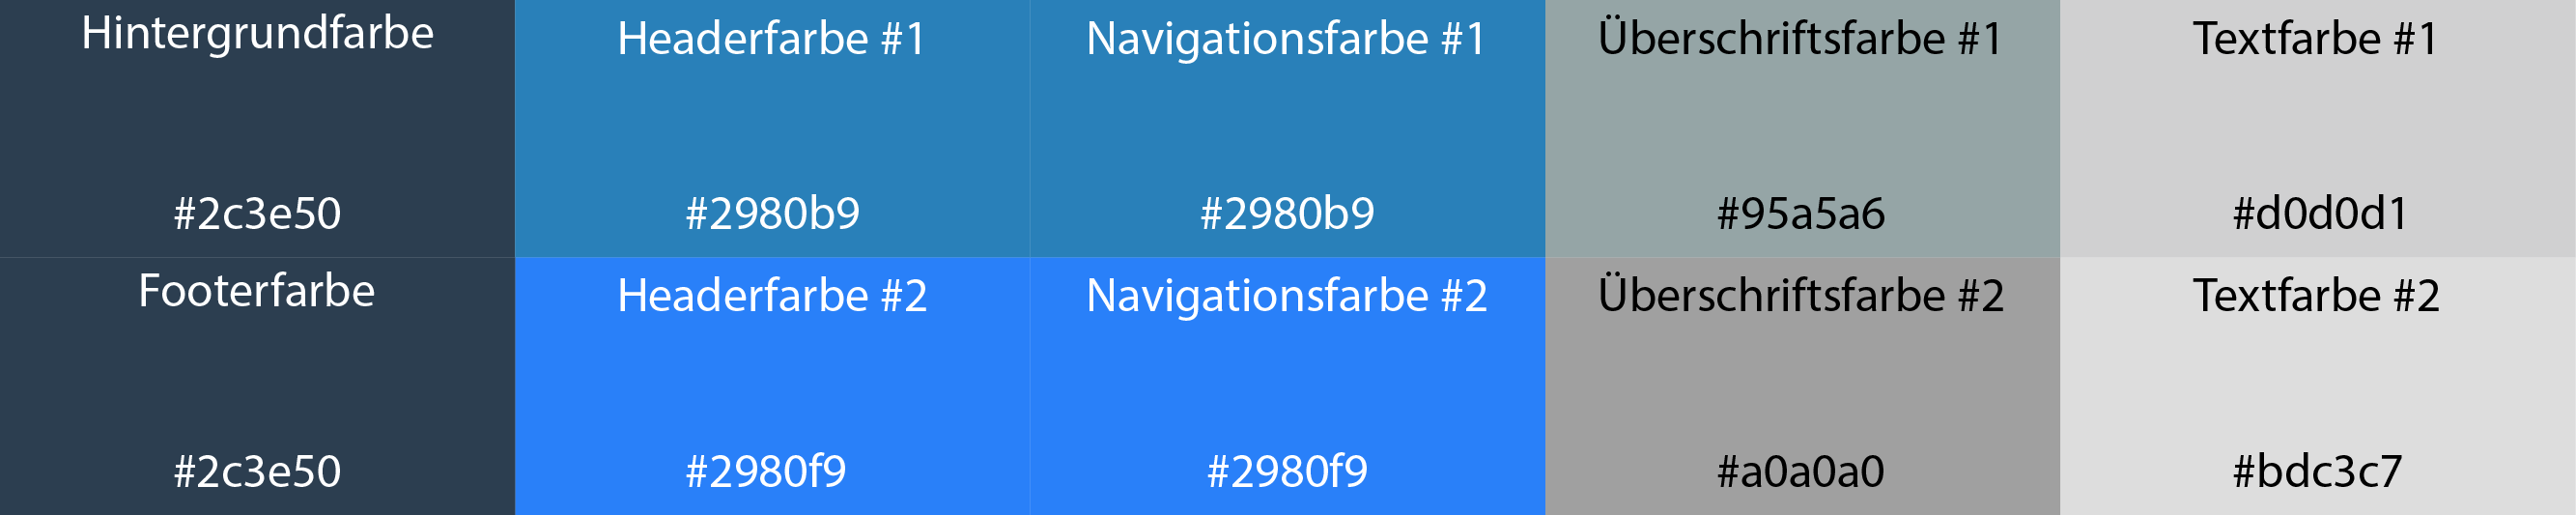
\includegraphics[width=\textwidth]{./img/mini_farb1.png}
\caption{Das Hauptfarbschema}
\label{mini_farb1}
\end{figure}

Als 1. alternatives Farbschema wurde ein geteilt komplementäres Farbschema gewählt. Dieses steht sehr zum Kontrast zum Hauptfarbschema. (siehe Abbildung \ref{mini_farb2}) 
\\
Die Hintergrundfarbe ist orange mit einem Gelbstich. Die ist positiv besetzt, und symbolisiert zudem Sonnenschein und Kreativität. Dadurch wirkt die ganze Shopseite auch ungezwungener, was bei der Vermarktung von Produkten auch wichtig ist. Zusätzlich vermittelt orange eine gute Wohnatmosphäre.
\\
Für den Header und die Navigationsleiste wird die Komplementärfarbe zu orange, blau, verwendet. Diese steht für Offenheit, Intelligenz und Vertrautheit. Dadurch passt es auch zu dem Angebot der digitalen Haustechnik. 
\\
Der Text ist in schwarz beziehungsweise dunklen Grautönen gehalten, und ist somit ein guter Kontrast zum Hintergrund. Zusätzlich drückt sie Eleganz und Stärke aus.

\begin{figure} [hp]
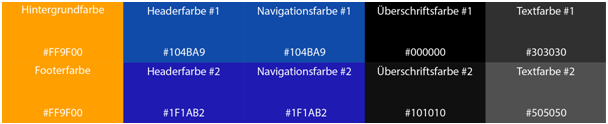
\includegraphics[width=\textwidth]{./img/mini_farb2.png}
\caption{Das 1. alternative Farbschema }
\label{mini_farb2}
\end{figure}

Als 2. alternatives Farbschema wurde ein komplementäres Farbschema gewählt. Dieses steht wieder sehr im Kontrast zum Hauptfarbschema. (siehe Abbildung \ref{mini_farb3})
\\
Die Hintergrundfarbe ist ein kräftiges Orange, was auch Kreativität und Sonne und dadurch auch Wärme symbolisiert. Zusätzlich ist sie positiv besetzt und drückt auch eine gemütliche Atmosphäre aus.
\\
Der Header und die Navigationsleiste sind in der Komplementärfarbe von dem orange, türkisblau,  gefärbt. Diese wirkt sehr lebendig und hat einen hohen Kontrast zu dem Hintergrund.
\\
Der Text ist in Grautönen, wodurch man den Inhalt sehr gut lesen kann. Zudem unterstreicht es den Minimalismus des Webseitenlayouts.

\begin{figure} [hp]
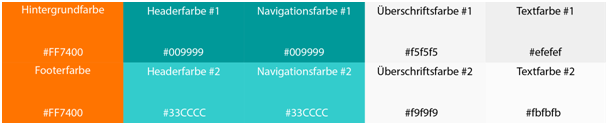
\includegraphics[width=\textwidth]{./img/mini_farb3.png}
\caption{Das 3. alternative Farbschema }
\label{mini_farb3}
\end{figure}

	\subsection{Typographische Gestaltung}\label{chapter:mini:typo}

Als Schriftart wurde die Schriftart „Raleway“ gewählt, da sie sehr innovativ und technisch wirkt. Diese unterstreicht das Minimalistische im Design. (für weitere Begründung vgl. Kapitel \ref{typo_inno} und Kapitel \ref{typo_zeit})
\\
Die Schriftgrößen sind möglichst groß gewählt, damit man den Inhalt der Seite sehr gut lesen kann.
\\
Die Schriftfarben sind so gewählt, das diese einen guten Kontrast zum Hintergrund bieten, und dadurch man eine hohe Lesbarkeit erreicht. (siehe Kapitel \ref{farb_mini})


	\subsection{Strukturanalyse der Seite}
Wie in Abbildung \ref{mini_comp3} zu sehen, beinhaltet der Header das Logo mit einem Werbespruch.
Die Navigation sitzt auf der rechten Seite, da diese Seite sich aus der Masse hervorheben soll, denn viele Seiten haben standardmäßig auf der linken Seite oder oben unterhalb des Headers ihre Navigationsleiste. Diese soll ein Drittel des Platzes auf der Webseite einnehmen, damit man die trotzdem sehr schnell erkennen kann. Zudem passt das vom Design her in den goldenen Schnitt. 
\\
Der Content soll zwischen Header und Footer sein, und wird horizontal von der Navigationsleiste eingeschränkt. Dabei soll er bei Textseiten so strukturiert sein, dass bei jedem Abschnitt ein Bild abwechselnd auf der linken und auf der rechten Seite hat. Somit wirkt es trotz des minimalistischem Designs nicht so eintönig. Auf Seiten mit vielen Bildern, zum Beispiel der Seite mit der Produktübersicht, sollen die Elemente tabellarisch und wegen dem Responsive Design auch dynamisch angeordnet sein.
\\
Der Footer enthält Informationen zum Copyright, dem Webseiten-Betreiber sowie ein Link zum Impressum.
